\documentclass[10pt]{jsarticle}%文字サイズが10ptのjsarticle

%%%%%%%%%%%%%%%%%%%%%%%%%%%%%%%%%%%%%%%%%%%%%%%%%%%%%%%
%%  パッケージ                                        %%
%%%%%%%%%%%%%%%%%%%%%%%%%%%%%%%%%%%%%%%%%%%%%%%%%%%%%%%
%使用しないときはコメントアウトしてください
\usepackage{amsthm}%定理環境
\usepackage{framed}%文章を箱で囲う
\usepackage{amsmath,amssymb}%数式全般
\usepackage{ascmac} % itembox環境 
\usepackage[dvipdfmx]{graphicx}%図の挿入
%\usepackage{tikz}%描画
\usepackage{titlesec}%見出しの見た目を編集できる
\usepackage[dvipdfmx, usenames]{color}%色をつける
%\usepackage{tikz-cd}%可換図式
%\usepackage{mathtools}%数式関連
\usepackage{amsfonts}%数式のフォント
\usepackage[all]{xy}%可換図式
\usepackage{mathrsfs}%花文字
\usepackage{comment}%コメント環境
\usepackage{picture}%お絵かき
\usepackage{url}%URLを出力
\usepackage{ulem}% 波線、打ち消し線
\usepackage{fancybox}%文章の囲み


%%% ↓コメント外すとリンクに色がつく
%\usepackage[dvipdfmx]{hyperref}
%\usepackage{pxjahyper}%日本語しおりの文字化けを防ぐ

\allowdisplaybreaks[1]%数式がページをまたぐことを許す

%ページ番号を右上に表記
\makeatletter
\def\@evenhead{\hfil\thepage}%
\def\@oddhead{\hfil\thepage}%
\def\@evenfoot{\@empty}%
\def\@oddfoot{\@empty}%
\makeatother


%%%%%%%%%%%%%%%%%%%%%%%%%%%%%%%%%%%%%%%%%%%%%%%%%%%%%%%
%%  表紙                                             %%
%%%%%%%%%%%%%%%%%%%%%%%%%%%%%%%%%%%%%%%%%%%%%%%%%%%%%%%
\makeatletter
\def\thickhrulefill{\leavevmode \leaders \hrule height 1pt\hfill \kern \z@}
\renewcommand{\maketitle}{\begin{titlepage}%
    \let\footnotesize\small
    \let\footnoterule\relax
    \parindent \z@
    \reset@font
    \null\vfil
    \begin{flushleft}
      \huge \@title
    \end{flushleft}
    \par
    \hrule height 4pt
    \par
    \begin{flushright}
      \LARGE \@author \par
    \end{flushright}
    \vskip 60\p@
    \vfil\null
    \begin{flushright}
        {\small \@date}%
    \end{flushright}
  \end{titlepage}%
  \setcounter{footnote}{0}%
}
\makeatother




%%%%%%%%%%%%%%%%%%%%%%%%%%%%%%%%%%%%%%%%%%%%%%%%%%%%%%%
%%  sectionの修飾                                     %%
%%%%%%%%%%%%%%%%%%%%%%%%%%%%%%%%%%%%%%%%%%%%%%%%%%%%%%%
%四角ではじめて下線付き
\titleformat{\section}[block]
{}{}{0pt}
{
  \colorbox{black}{\begin{picture}(0,10)\end{picture}}
  \hspace{0pt}
  \normalfont \Large\bfseries
  \hspace{-4pt}
}
[
\begin{picture}(100,0)
  \put(3,18){\color{black}\line(1,0){300}}
\end{picture}
\\
\vspace{-30pt}
]

%subsubsectionの編集
\renewcommand{\thesubsubsection}{\textbf{問\arabic{subsubsection}}}%問(さぶさぶせくしょん番号)を出力






%%%%%%%%%%%%%%%%%%%%%%%%%%%%%%%%%%%%%%%%%%%%%%%%%%%%%%%
%%  番号付き定理環境                                  %%
%%%%%%%%%%%%%%%%%%%%%%%%%%%%%%%%%%%%%%%%%%%%%%%%%%%%%%%
%注:defというコマンドはもうある
\theoremstyle{definition}%定理環境のアルファベットを斜体にしない
\renewcommand{\proofname}{\textgt{証明}}%proof環境の修正

%%%%%%%%%%%%%%%%%%%%%%%%%%%%%%%%%%%%%%%%%%%%%%%%%%%%%%%
%%  番号なし定理環境                                  %%
%%%%%%%%%%%%%%%%%%%%%%%%%%%%%%%%%%%%%%%%%%%%%%%%%%%%%%%
%一部箱付き
\newtheorem*{lemma}{補題}
\newtheorem*{proposition}{命題}
\newtheorem*{definition}{定義}
\newcommand{\lem}[1]{\begin{oframed} \begin{lemma} #1 \end{lemma} \end{oframed}}%箱付きほだい
\newcommand{\prop}[1]{\begin{oframed} \begin{proposition} #1 \end{proposition} \end{oframed}}%箱付きめいだい

\newtheorem*{com}{コメント}
\newtheorem*{claim}{主張}
\newtheorem*{sol}{解答}
\newtheorem*{prob}{問題}
\newtheorem*{quo}{引用}
\newtheorem*{rem}{注意}



%%%%%%%%%%%%%%%%%%%%%%%%%%%%%%%%%%%%%%%%%%%%%%%%%%%%%%%
%%  左側に線を引く                                  %%
%%%%%%%%%%%%%%%%%%%%%%%%%%%%%%%%%%%%%%%%%%%%%%%%%%%%%%%
%leftbar環境の定義
\makeatletter
\renewenvironment{leftbar}{%
%  \def\FrameCommand{\vrule width 3pt \hspace{10pt}}%  デフォルトの線の太さは3pt
  \renewcommand\FrameCommand{\vrule width 1pt \hspace{10pt}}%
  \MakeFramed {\advance\hsize-\width \FrameRestore}}%
 {\endMakeFramed}
\newcommand{\exbf}[2]{ \begin{leftbar} \textbf{#1} #2 \end{leftbar} }%左線つき太字
%\newcommand{\barquo}[1]{\begin{leftbar} \begin{quo} #1 \end{quo} \end{leftbar}}%左線つき引用%びふぉあ
\newcommand{\barquo}[1]{\begin{leftbar} \noindent #1  \end{leftbar}}%左線つき引用
\newcommand{\lbar}[1]{\begin{leftbar} #1 \end{leftbar}}



%%%%%%%%%%%%%%%%%%%%%%%%%%%%%%%%%%%%%%%%%%%%%%%%%%%%%%%
%%  色をつける                                      %%
%%%%%%%%%%%%%%%%%%%%%%%%%%%%%%%%%%%%%%%%%%%%%%%%%%%%%%%
\newcommand{\textblue}[1]{\textcolor{blue}{\textbf{#1}}}

%%%%%%%%%%%%%%%%%%%%%%%%%%%%%%%%%%%%%%%%%%%%%%%%%%%%%%%
%%  よく使う記号の略記                                 %%
%%%%%%%%%%%%%%%%%%%%%%%%%%%%%%%%%%%%%%%%%%%%%%%%%%%%%%%
\newcommand{\setmid}[2]{\left\{ #1 \mathrel{} \middle| \mathrel{} #2 \right\}}%集合の内包記法
\newcommand{\sm}{\setminus}%集合差
\newcommand{\abs}[1]{\left \lvert #1 \right \rvert}%絶対値
\newcommand{\norm}[1]{\left \lVert #1 \right \rVert}%ノルム
\newcommand{\transpose}[1]{\, {\vphantom{#1}}^t\!{#1}}%行列の転置
\newcommand{\pmat}[1]{ \begin{pmatrix} #1 \end{pmatrix} }%まるかっこ行列
\newcommand{\f}[2]{\frac{#1}{#2}}%分数
\newcommand{\kakko}[1]{ \langle #1  \rangle}%鋭角かっこ%\angleはもうある
\newcommand{\I}{\sqrt{-1}}%虚数単位。\iは既にある。
\newcommand{\single}{\{ 0 \}}%0のシングルトン
\newcommand{\clsub}{\subset_{\text{closed}}}%閉部分集合
\newcommand{\opsub}{\subset_{\text{open}}}%開部分集合
\newcommand{\clirr}{\subset_{\text{closed irr}}}%閉既約部分集合
\newcommand{\loc}{\subset_{\text{loc. closed}}}%局所閉部分集合
\newcommand{\wt}[1]{\widetilde{#1}}%わいどちるだあ
\newcommand{\ol}[1]{\overline{#1}}%オーバーライン
\newcommand{\wh}[1]{\widehat{#1}}%ワイドハット
\newcommand{\To}{\Rightarrow}%ならば%自然変換
\newcommand{\xto}[1]{\xrightarrow}%上側文字付き右向き矢印
\newcommand{\st}{\; \; \text{s.t.} \; \;}%空白付きsuch that
\newcommand{\ts}{\otimes}%テンソル積
\newcommand{\tm}{\times}%直積
\newcommand{\vartm}{\times^{\text{Var}}}%多様体の圏における直積。集合の直積と区別するとき用。
\newcommand{\la}{\overleftarrow}%上付き左矢印
\newcommand{\ra}{\overrightarrow}%上付き右矢印
\newcommand{\del}{\partial}%偏微分の記号
\newcommand{\PD}[2]{  \frac{\partial #1}{\partial #2}  }%偏微分でるでる
\newcommand{\zyu}[1]{ \mathbb{Z} / #1 \mathbb{Z} }%有限巡回群
\newcommand{\s}[1]{ \sqrt{#1} }%平方根記号
\newcommand{\sh}{\mathbin{\sharp}}%シャープ%良い子の諸君!このシャープは二項演算として定義したので、ただのシャープではないことに注意だ
\newcommand{\id}{\mathrm{id}}%アイデンティティ



%%%%%%%%%%%%%%%%%%%%%%%%%%%%%%%%%%%%%%%%%%%%%%%%%%%%%%%
%%       演算子                                       %%
%%%%%%%%%%%%%%%%%%%%%%%%%%%%%%%%%%%%%%%%%%%%%%%%%%%%%%%
%log型
\DeclareMathOperator{\rank}{rank}%行列の階数
\DeclareMathOperator{\rk}{rk}%行列の階数
\DeclareMathOperator{\corank}{corank}%行列の核の次元
\renewcommand{\Re}{\operatorname{Re}}%実部
\DeclareMathOperator{\Res}{Res}%留数
\DeclareMathOperator{\Gal}{Gal}%Galois群
\DeclareMathOperator{\Hom}{Hom}%射の集合
\DeclareMathOperator{\ind}{Ind}
\DeclareMathOperator{\tr}{tr}%トレース
\DeclareMathOperator{\Tr}{Tr}%トレース
\DeclareMathOperator{\Norm}{N}%ノルム
\DeclareMathOperator{\Aut}{Aut}%自己同型群
\DeclareMathOperator{\trdeg}{tr\text{.}deg}%超越次数
\DeclareMathOperator{\Frac}{Frac}%商体をとる操作
\renewcommand{\Im}{\operatorname{Im}}%写像の像。Abel圏の像対象。虚部が出力できなくなった。
\DeclareMathOperator{\Ker}{Ker}%写像の核。Abel圏の核対象。
\DeclareMathOperator{\im}{im}%写像の像
\DeclareMathOperator{\coker}{coker}%余核%対象のほう
\DeclareMathOperator{\Coker}{Coker}%余核%射のほう
\DeclareMathOperator{\Spec}{Spec}%スペクトル
\DeclareMathOperator{\Sing}{Sing}%Singular point.特異点の集合。歌ってるわけではないぞ
\DeclareMathOperator{\Supp}{Supp}%台
\DeclareMathOperator{\ann}{ann}%アナイアレーター
\DeclareMathOperator{\Ass}{Ass}%素因子
\DeclareMathOperator{\ord}{ord}%おーだー
\DeclareMathOperator{\height}{ht}%素イデアルの高度。\htはもうある
\DeclareMathOperator{\coht}{coht}%素イデアルの余高度
\DeclareMathOperator{\Lan}{Lan}%左Kan拡張
\DeclareMathOperator{\Ran}{Ran}%右Kan拡張
\DeclareMathOperator{\Orbit}{Orbit}%作用の軌道
\DeclareMathOperator{\Stab}{Stab}%作用の安定化群
\DeclareMathOperator{\sgn}{sgn}%符号


%limit型
\DeclareMathOperator*{\llim}{\varprojlim}%極限。逆極限。射影極限。
\DeclareMathOperator*{\rlim}{\varinjlim}%余極限。順極限。入射極限。

%%%%%%%%%%%%%%%%%%%%%%%%%%%%%%%%%%%%%%%%%%%%%%%%%%%%%%%
%%  黒板太字(blackboard bold)                         %%
%%%%%%%%%%%%%%%%%%%%%%%%%%%%%%%%%%%%%%%%%%%%%%%%%%%%%%%
\newcommand{\bba}{{\mathbb A}}
\newcommand{\bbb}{{\mathbb B}}
\newcommand{\bbc}{{\mathbb C}}
\newcommand{\bbd}{{\mathbb D}}
\newcommand{\bbe}{{\mathbb E}}
\newcommand{\bbf}{{\mathbb F}}
\newcommand{\bbg}{{\mathbb G}}
\newcommand{\bbh}{{\mathbb H}}
\newcommand{\bbi}{{\mathbb I}}
\newcommand{\bbj}{{\mathbb J}}
\newcommand{\bbk}{{\mathbb K}}
\newcommand{\bbl}{{\mathbb L}}
\newcommand{\bbm}{{\mathbb M}}
\newcommand{\bbn}{{\mathbb N}}
\newcommand{\bbo}{{\mathbb O}}
\newcommand{\bbp}{{\mathbb P}}
\newcommand{\bbq}{{\mathbb Q}}
\newcommand{\bbr}{{\mathbb R}}
\newcommand{\bbs}{{\mathbb S}}
\newcommand{\bbt}{{\mathbb T}}
\newcommand{\bbu}{{\mathbb U}}
\newcommand{\bbv}{{\mathbb V}}
\newcommand{\bbw}{{\mathbb W}}
\newcommand{\bbx}{{\mathbb X}}
\newcommand{\bby}{{\mathbb Y}}
\newcommand{\bbz}{{\mathbb Z}}

%%%%%%%%%%%%%%%%%%%%%%%%%%%%%%%%%%%%%%%%%%%%%%%%%%%%%%%
%%  よく使う黒板太字                                  %%
%%%%%%%%%%%%%%%%%%%%%%%%%%%%%%%%%%%%%%%%%%%%%%%%%%%%%%%
\newcommand{\Z}{\bbz}%整数
\newcommand{\A}{\bba}
\newcommand{\Q}{\bbq}%有理数
\newcommand{\R}{\bbr}%実数
\newcommand{\C}{\bbc}%複素数
\newcommand{\F}{\bbf}%有限体
\newcommand{\N}{\bbn}%自然数
\newcommand{\T}{\bbt}%トーラス
\renewcommand{\P}{\bbp}%パラグラフ記号が出力できなくなった%射影空間

%%%%%%%%%%%%%%%%%%%%%%%%%%%%%%%%%%%%%%%%%%%%%%%%%%%%%%%
%%  カリグラフィー                                %%
%%%%%%%%%%%%%%%%%%%%%%%%%%%%%%%%%%%%%%%%%%%%%%%%%%%%%%%
%大文字しかどうせ使わない
\newcommand{\cala}{\mathcal{A}}
\newcommand{\calb}{\mathcal{B}}
\newcommand{\calc}{\mathcal{C}}
\newcommand{\cald}{\mathcal{D}}
\newcommand{\calf}{\mathcal{F}}
\newcommand{\calo}{\mathcal{O}}

%%%%%%%%%%%%%%%%%%%%%%%%%%%%%%%%%%%%%%%%%%%%%%%%%%%%%%%
%%  ギリシャ文字(Greek letters)小文字                 %%
%%%%%%%%%%%%%%%%%%%%%%%%%%%%%%%%%%%%%%%%%%%%%%%%%%%%%%%
%コマンドが5字以上のもの
\newcommand{\gra}{{\alpha}}
\newcommand{\grg}{{\gamma}}
\newcommand{\grd}{{\delta}}
\newcommand{\gre}{{\epsilon}}
\newcommand{\grt}{{\theta}}
\newcommand{\grk}{{\kappa}}
\newcommand{\grl}{{\lambda}}
\newcommand{\grs}{{\sigma}}
\newcommand{\gru}{{\upsilon}}
\newcommand{\gro}{{\omega}}

\newcommand{\ve}{{\varepsilon}}
\newcommand{\vp}{{\varphi}}

%%%%%%%%%%%%%%%%%%%%%%%%%%%%%%%%%%%%%%%%%%%%%%%%%%%%%%%
%%  ギリシャ文字(Greek letters)大文字                 %%
%%%%%%%%%%%%%%%%%%%%%%%%%%%%%%%%%%%%%%%%%%%%%%%%%%%%%%%
%コマンドが5字以上のもの
\newcommand{\grG}{{\Gamma}}
\newcommand{\grD}{{\Delta}}
\newcommand{\grT}{{\Theta}}
\newcommand{\grL}{{\Lambda}}
\newcommand{\grS}{{\Sigma}}
\newcommand{\grU}{{\Upsilon}}
\newcommand{\grO}{{\Omega}}

%%%%%%%%%%%%%%%%%%%%%%%%%%%%%%%%%%%%%%%%%%%%%%%%%%%%%%%
%%  フラクトゥール                                  %%
%%%%%%%%%%%%%%%%%%%%%%%%%%%%%%%%%%%%%%%%%%%%%%%%%%%%%%%
\newcommand{\fraka}{\mathfrak{a}}
\newcommand{\frakb}{\mathfrak{b}}
\newcommand{\frakm}{\mathfrak{m}}
\newcommand{\frakn}{\mathfrak{n}}
\newcommand{\frakp}{\mathfrak{p}}
\newcommand{\frakq}{\mathfrak{q}}

\newcommand{\frakA}{\mathfrak{A}}
\newcommand{\frakB}{\mathfrak{B}}
\newcommand{\frakS}{\mathfrak{S}}
\newcommand{\frakT}{\mathfrak{T}}

\newcommand{\Top}{\mathfrak{Top}}%開部分集合全体のなす有向集合
\newcommand{\Ab}{\mathfrak{Ab}}%Abel群のなす圏

%%%%%%%%%%%%%%%%%%%%%%%%%%%%%%%%%%%%%%%%%%%%%%%%%%%%%%%
%%  花文字                                          %%
%%%%%%%%%%%%%%%%%%%%%%%%%%%%%%%%%%%%%%%%%%%%%%%%%%%%%%%
%大文字しかどうせ使わない
\newcommand{\scra}{\mathscr{A}}
\newcommand{\scrf}{\mathscr{F}}
\newcommand{\scrg}{\mathscr{G}}
\newcommand{\scrh}{\mathscr{H}}
\newcommand{\scrs}{\mathscr{S}}

%%%%%%%%%%%%%%%%%%%%%%%%%%%%%%%%%%%%%%%%%%%%%%%%%%%%%%%
%%  太字                                            %%
%%%%%%%%%%%%%%%%%%%%%%%%%%%%%%%%%%%%%%%%%%%%%%%%%%%%%%%
\newcommand{\Sh}{\textbf{Sh}}%層の圏
\newcommand{\PSh}{\textbf{PSh}}%前層の圏
\newcommand{\bfzero}{\textbf{0}}%太字のゼロ

%小文字
\newcommand{\bfb}{\textbf{b}}
\newcommand{\bfu}{\textbf{u}}
\newcommand{\bfv}{\textbf{v}}
\newcommand{\bfx}{\textbf{x}}
\newcommand{\bfy}{\textbf{y}}


%大文字
\newcommand{\bfC}{\textbf{C}}
\newcommand{\bfD}{\textbf{D}}
\newcommand{\bfE}{\textbf{E}}



\setcounter{tocdepth}{3}%目次に含めるレベル。1ならsectionまで。2ならsubsectionまで。3ならsubsubsectionまで。
\begin{document}



\title{年金2次 \; 簡記問題集 \; DC編}
\author{hyaraguchi}
\date{\today}
\maketitle


\tableofcontents%目次

\newpage

%\section{はじめに}


%\newpage

% 企業型年金の開始
\section{企業型年金の開始}





\newpage



% 企業型年金加入者等
\section{企業型年金加入者等}

%1節 企業型年金加入者
\subsubsection{加入可能年齢の変更}
\barquo{
  「年金制度の機能強化のための国民年金法等の一部を改正する法律」(令和 2 年6 月5 日公
  布)により確定拠出年金の加入可能要件の見直し等が実施されることに関し、次の(a)およ
  び(b)の内容を簡記しなさい。

  \begin{enumerate}
    \renewcommand{\labelenumi}{(\alph{enumi})}
    \item 令和 4 年 5 月1 日施行の企業型年金における加入可能年齢の変更について
    \item 令和 4 年 5 月1 日施行の個人型年金における加入可能年齢の変更について
  \end{enumerate}

  \rightline{引用元:年金1 2020 問2(2)\textcircled{3}}
}

\begin{itembox}[l]{\textgt{ポイント}}
  令和2年6月の法改正による加入要件緩和に関する問題。

  \begin{center}
    \begin{tabular}{l|cc} 
      \hline
      & 法改正前 & 法改正後  \\
      \hline \hline
      企業型年金(法第9条) & 
        \begin{tabular}{c}
        厚生年金保険の被保険者 \\
        のうち65歳未満の者
        \end{tabular} 
      & \textcolor{red}{厚生年金保険の被保険者} \\ \hline
      個人型年金(法第62条) & 
        \begin{tabular}{c}
        国民年金の被保険者 \\
        のうち60歳未満の者
        \end{tabular}
      & \textcolor{red}{国民年金の被保険者}\\
    \end{tabular}
  \end{center}
\end{itembox}

\begin{sol}
  \;

  \begin{enumerate}
    \renewcommand{\labelenumi}{(\alph{enumi})}
    \item 令和4年5月1日施行以前は、厚生年金保険の被保険者のうち65歳未満の者しか企業型年金に
      加入できなかったが、施行後は厚生年金保険の被保険者であれば加入者となることができるようになった。
    \item 令和4年5月1日施行以前は、国民年金の被保険者のうち60歳未満の者しか個人型年金に
    加入できなかったが、施行後は国民ねんきんの被保険者であれば個人型年金に加入可能になった。
  \end{enumerate}
\end{sol}

\newpage

\subsubsection{一定の資格}
\barquo{
  企業型年金加入者となることについて「一定の資格」として定めることができる4 つの資格
  および、当該「一定の資格」を定める場合に、企業型年金加入者とならない従業員に対して基
  本的には適用されていることが必要とされる措置(代替措置)について簡記しなさい。

  \rightline{引用元:年金1 2019 問2(4)\textcircled{1}}
}

\begin{itembox}[l]{\textgt{ポイント}}
  解釈第1-1。
  一定の資格として定めることができる要件は以下の通り。
  \begin{enumerate}
    \item 一定の職種
    \item 一定の勤続期間
    \item 一定の年齢
    \item 希望するもの
  \end{enumerate}
  加入除外された者へは以下の代替措置を設ける必要がある。
  \begin{itemize}
    \item 「一定の職種」「一定の勤続期間」
    \begin{itemize}
      \item イメージはすでに他制度がある場合の代替措置。
      \item 厚生年金基金、DB、退職一時金制度(前払い退職金制度も含む)に加入し続けることが代替措置になる。
    \end{itemize}
    \item 「一定の年齢」「希望する者」
    \begin{itemize}
      \item どちらかといえば、新たにDCを実施する場合の代替措置。
      \item 退職一時金制度(前払い一時金制度も含む)に加入し続けることが代替措置になる。
      \item 「希望する者」の場合は、DBに加入することでもよい。
    \end{itemize}
  \end{itemize}
\end{itembox}

\begin{sol}
  \;

  企業型年金加入者となることについて定めることができる資格とは、
  \begin{enumerate}
    \item 一定の職種
    \item 一定の勤続年数
    \item 一定の年齢
    \item 希望する者
  \end{enumerate}
  の四つである。

  このうち1、2については、厚生年金基金(加算部分)、確定給付企業年金または退職一時金制度
  (前払い一時金制度も含む)が適用されていることが代替措置となる。
  また、3、4については、確定給付企業年金(4の場合のみ)または退職一時金制度
  (前払い一時金制度も含む)が適用されていることが代替措置となる。


\end{sol}

\newpage


%2節 資格取得の時期
\subsubsection{資格取得の時期}
\barquo{
  確定拠出年金法第10条に記載されている企業型年金加入者の資格取得時期をすべて列挙しなさい。

  \rightline{(自作)}
}

\begin{itembox}[l]{\textgt{ポイント}}
  DBの資格取得時期とまったく同じ。
\end{itembox}

\begin{sol}
  \;

  以下の4点。
  \begin{itemize}
    \item 実施事業所に使用されるに至ったとき。
    \item その使用されている事業所もしくは事務所または船舶が、実施事業所になったとき。
    \item 実施事業所に使用されている者が、厚生年金保険の被保険者となったとき。
    \item 実施事業所に使用されている者が、企業型年金規約に定める資格を取得したとき。
  \end{itemize}
\end{sol}

\newpage


% 掛金
\section{掛金}

% 1節 事業主掛金
\subsubsection{事業主掛金の年単位化}
\barquo{
  以下のBさんについて、(a)、(b)それぞれにおける金額を入力しなさい。なお、算出
  過程についても入力すること。 ((a)、(b)それぞれ100 字以内)

  \;

  <Bさんの情報>
  \begin{itemize}
    \item 企業型年金に加入しており、確定拠出年金法施行令に規定する他制度加入者、個人型年金同時加入可能者のいずれにも該当しない
    \item 企業型年金加入者掛金の拠出はない
    \item Bさんが加入している企業型年金の拠出区分期間は3か月(年4回(3月、6月、9月、12月)の各月に前月までの分の事業主掛金を拠出)である
  \end{itemize}
  
  \begin{enumerate}
    \renewcommand{\labelenumi}{(\alph{enumi})}
    \item 2022 年(令和4 年)12 月に60,000 円(月額ベースで20,000 円)、2023 年(令和5 年)
      3 月に60,000 円(月額ベースで20,000 円)の事業主掛金を拠出した場合の2023 年(令和
      5 年)6 月における事業主掛金の最大額
    \item 2023 年(令和5 年)3 月に60,000 円(月額ベースで20,000 円)、2023 年(令和5 年)6
      月に60,000 円(月額ベースで20,000 円)、2023 年(令和5 年)9 月に80,000 円(月額ベ
      ース20,000 円に加え賞与のあった6 月分は20,000 円を加算)の事業主掛金を拠出した場
      合の2023 年(令和5 年)12 月における事業主掛金の最大額
  \end{enumerate}

  \rightline{引用元:年金1 2023 問2(2)(ウ) }
}

\begin{itembox}[l]{\textgt{ポイント}}
  法第19条。
  2018年1月1日施行で、事業主掛金を\textcolor{red}{年単位}で拠出することが可能になった。

  \;

  \begin{center}
    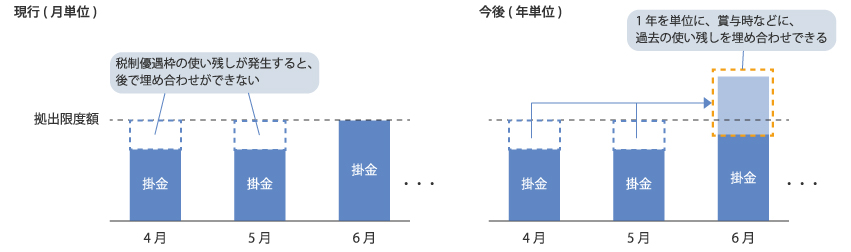
\includegraphics[width=130mm]{figure/nentanika.jpg}
  \end{center}

  \rightline{図の引用元:\url{https://kumitateru.jp/media/topic/a46} }

  
  年単位化により比較的自由に事業主掛金を拠出できるようになったが、以下のようなルールが存在する。

  \begin{itemize}
    \item その月までの拠出限度額を超えてはいけない(令第11条の2)
    \item 拠出区分期間の変更は年1回まで(解釈第1-2.(7))
  \end{itemize}
  
\end{itembox}

\begin{sol}
  \;

  \begin{enumerate}
    \renewcommand{\labelenumi}{(\alph{enumi})}
    \item 2023年6月時点で拠出可能な事業主掛金の総額は、$55,000(円) \times 6(月) = 330,000(円)$。
    
    2023年6月時点で実際に拠出している事業主掛金は、2023年3月拠出の$60,000$(円)。

    したがって、2023年6月に拠出できる事業主掛金の最大額は、$330,000(円)- 60,000(円)=\textcolor{red}{270,000(円)}$。
    
    \item 2023年12月時点で拠出可能な事業主掛金の総額は、$55,000(円) \times 12(月) = 660,000(円)$。

    2023年12月時点で実際に拠出している事業主掛金は、2023年3、6、9月に拠出した事業主掛金の合計額なので、
    $60,000(円)+60,000(円)+80,000(円) = 200,000(円)$。

    したがって、2023年12月に拠出できる事業主掛金の最大額は、$660,000(円)-200,000(円)=\textcolor{red}{460,000(円)}$。

  \end{enumerate}
\end{sol}

\newpage

\subsubsection{事業主掛金の算定方法:不当に差別的なもの}
\barquo{
  確定拠出年金法施行令第6 条第2 号において、事業主掛金の額の算定方法等は、特定の者に
  ついて不当に差別的なものでないこととされている。また、同条第4 号において、企業型年
  金加入者が掛金を拠出することができることを企業型年金規約に定める場合の要件が定めら
  れており、企業型年金加入者掛金の額の決定又は変更の方法は、特定の者について不当に差
  別的なものでないこととされている。

  この「不当に差別的なものでないこと」に該当しないものとして『確定拠出年金法並びにこ
  れに基づく政令及び省令について(法令解釈)』に例示されているものを2 つ簡潔に入力しな
  さい。

  \rightline{引用元:年金1 2022 問2(2)(ア)}
}

\begin{itembox}[l]{\textgt{ポイント}}
  解釈第1-3.(7)の内容をそのまま入力すればよい。
\end{itembox}

\begin{sol}
  \;
  \begin{enumerate}
    \item 一定の資格(職種・勤続期間・年齢)を設けて、企業年金加入者掛金の額または拠出区分期間の
      決定または変更方法に差を付けること。
    \item 事業主返還において、企業型年金加入者掛金の拠出があるにもかかわらず企業型年金加入者
      であった者への返還額が零であること。
  \end{enumerate}
\end{sol}

\newpage


%2節 選択制DC
\subsubsection{選択制DC:従業員への説明}
\barquo{
  『確定拠出年金法並びにこれに基づく政令及び省令について(法令解釈)』に定める、労使合
  意により給与等を減額した上で、当該減額部分を事業主掛金として拠出し企業型年金の個人別
  管理資産として積み立てるか、給与等への上乗せで受け取るかを従業員が選択する仕組みを実
  施するに当たって、事業主が従業員に正確な説明を行う必要がある内容に含まれるものについ
  て簡記しなさい。

  \rightline{引用元:年金1 2021 問2(2)\textcircled{1}}
}

\begin{itembox}[l]{\textgt{ポイント}}
  Q\&A70。

  選択制DCを導入する際、下記の点を従業員に説明する必要がある。

  \begin{itemize}
    \item 社会保険・雇用保険等の給付が減額する可能性があること。
  \end{itemize}
\end{itembox}

\begin{sol}
  \;
  
  給与等を減額して事業主掛金を拠出した場合、社会保険・雇用保険等の給付額が減額する可能性がある点について、
  事業主は従業員に正確な説明を行う必要がある。

\end{sol}

\newpage

%3節 企業型年金加入者掛金
\subsubsection{企業型年金加入者掛金:不当に制約されるものではないこと}
\barquo{
  企業型年金加入者が掛金を拠出することができることを企業型年金規約に定める場合にあっ
  ては、確定拠出年金法施行令第 6 条第4 号ニのとおり企業型年金加入者掛金の額の決定または
  変更の方法その他その拠出に関する事項が事業主によって不当に制約されるものでないことが
  必要であるが、 『確定拠出年金法並びにこれに基づく政令及び省令について(法令解釈) 』に示
  されている、「不当に制約されるものでないこと」に該当しない例を2つ簡記しなさい。

  \rightline{引用元:年金1 2020 問2(2)\textcircled{2}}
}

\begin{itembox}[l]{\textgt{ポイント}}
  「不当に制約されるものでないこと」は解釈第1-3.(8)に例示されている。
  ここで例示されているケースは、加入者の意思を反映してるとは言えず、法令で制限されている。
\end{itembox}

\begin{sol}
  \;
  
  \begin{itemize}
    \item 企業型年金加入者掛金の額または拠出区分期間の指定がなかった者は、
      特定の企業型年金加入者掛金の額または拠出区分期間を選択したものとすること。
    \item 企業型年金加入者掛金の額が毎年自動的に増加または減少することを設けること。
  \end{itemize}
\end{sol}

\newpage

\subsubsection{加入者掛金の変更}
\barquo{
  以下の記述の正誤を判定し、誤っている場合はその理由を簡記しなさい。

  \;

  企業型年金へ加入者掛金を拠出している加入者が、事業主掛金が変わらず、かつ加入者の
  資格も喪失しない状況で、企業型掛金拠出単位期間に1回を超えて加入者掛金を変更するこ
  とができるのは、加入者掛金を零に変更する場合だけである。

  \rightline{引用元:年金1 2018 問2(2)\textcircled{3}}
}

\begin{itembox}[l]{\textgt{ポイント}}
  令第6条第1項第4号ハ。則第4条の2。

  マッチング拠出の掛金額は\textcolor{red}{原則年1回}(厳密には拠出単位期間に1回)しか変更できないが、
  以下に該当する場合は例外として「年1回ルール」とは別に掛金額変更が認められている。
  \begin{itemize}
    \item 「事業主掛金」の超過を回避するための変更
    \item 「拠出限度額 $-$ 事業主掛金額」の超過を回避するための変更
    \item 0円への変更
    \item 0円からの変更
    \item マッチング拠出額の選択肢が変更されることにより、今まで拠出していた金額が選択肢から除外された場合
    \item \textcolor{red}{事業主掛金額または他制度掛金相当額が引き下がる場合において、当該企業型年金の加入者掛金を引き上げる場合}(令和6年12月1日施行)
  \end{itemize}

\end{itembox}

\begin{sol}
  \;

  正。

  \begin{shadebox}
    (令和6年12月1日以降の回答)
    
    誤。

    他制度掛金相当額が引き下がった時に加入者掛金を引き上げる場合も、
    企業型掛金拠出単位期間に1回を超えて加入者掛金を変更できる。
  \end{shadebox}
  
\end{sol}

\newpage


%他制度掛金相当額
\section{他制度掛金相当額}

%1節 他制度掛金相当額の見直し
\subsubsection{他制度掛金相当額:加入者掛金の取り扱い}
\barquo{
  通知「確定拠出年金における他制度掛金相当額及び共済掛金相当額の算定方法について(令
  和3 年9 月1 日年企発第0901 第2 号)」に定める、加入者が掛金の一部を負担している場合
  の他制度掛金相当額及び共済掛金相当額にかかる取扱いについて簡潔に入力しなさい。な
  お、 「確定給付企業年金制度の場合」と「確定給付企業年金制度以外の他制度の場合」のそれ
  ぞれについて入力すること。また、制度内容に応じた具体的な算定方法には触れなくてよ
  い。 (250 字以内)

  \rightline{引用元:年金1 2023 問2(2)(イ) }
}

\begin{itembox}[l]{\textgt{ポイント}}
  算定省令第5条の理解を問う問題。

  DBでは、他制度掛金相当を算定する際、加入者負担掛金を\textcolor{red}{零}とみなして算定するが、
  DB以外の他制度の場合は、\textcolor{red}{加入者負担掛金も含めて算定する}必要がある。

  実務的には、加入者が掛金を負担している給付区分にかかる他制度掛金相当額を0円にするなど、
  合理的な方法で算定するようにしなければならない。
\end{itembox}

\begin{sol}
  \;

  「確定給付企業年金制度の場合」

   加入者が負担する掛金は零であるものとして算定する。

  「確定給付企業年金制度以外の他制度の場合」

  加入者が負担する掛金も含めて算定する。
\end{sol}

\newpage

%2節 他制度掛金相当額の算定
\subsubsection{他制度掛金相当額の算定にかかる経過措置}
\barquo{
  「確定拠出年金における他制度掛金相当額及び共済掛金相当額の算定に関する省令(令和3 年厚
  生労働省令第150 号)」において定められている、2024 年(令和6 年)12 月1 日前を計算基
  準日とする財政計算の結果に基づいて掛金の額を算定する事業主等の確定給付企業年金の加
  入者に係る他制度掛金相当額に関する経過措置について簡潔に入力しなさい。なお、リスク
  分担型企業年金以外である場合についてのみ入力すること。

  \rightline{引用元:年金1 2022 問2(2)(イ) }
}

\begin{itembox}[l]{\textgt{ポイント}}
  算定省令附則第2条。2024年12月1日以前を計算基準日とする財政計算で他制度掛金を算定する場合、
  経過措置として、簡易型DBと同じ方法で他制度掛金を算定できる。
  解答には、簡易型DBの他制度掛金算定方法を入力すればよい。
\end{itembox}

\begin{sol}
  \;

  直近の財政計算の基準日における当該財政計算の結果に基づく標準掛金額を当該財政計算の
  計算基準日における加入者の数で除した額を1月あたりの額に換算した額とすることができる。
\end{sol}

\newpage

\subsubsection{休職等の取り扱い}
\barquo{
  通知「確定拠出年金における他制度掛金相当額及び共済掛金相当額の算定方法について(令
  和3 年9 月1 日年企発第0901 第2 号)」において定められている、一部の加入者の確定給付
  企業年金の掛金拠出がない場合(※)における、当該加入者に係る他制度掛金相当額の取り
  扱いについて簡潔に入力しなさい。

  (※)確定給付企業年金に加入している休職者であって、掛金の拠出を中断する取扱いや一
  定の年齢以降を給付の額の算定の基礎としていない等によるもの。

  \rightline{引用元:年金1 2022 問2(2)(ウ) }
}

\begin{itembox}[l]{\textgt{ポイント}}
  休職等の取り扱いについては、Q\&A15,16に記載がある。

  一部の加入者について掛金の拠出がない場合も、他制度掛金相当額は零円ではなく、
  \textcolor{red}{他の加入者と同額}を設定しなければならない。
\end{itembox}

\begin{sol}
  \;

  掛金拠出や給付の額の算定の基礎の取り扱いにかかわらず、確定給付企業年金の加入者である以上、
  当該確定給付企業年金の他の加入者と同じ金額を設定する必要がある。
\end{sol}

\newpage

% 運用

% 給付
\section{給付}


%2節 老齢給付金
\subsubsection{老齢給付金の支給要件:通算加入者期間}
\barquo{
  確定拠出年金法第33条第1項に定める、老齢給付金の支給の請求に関する通算加入者等期
  間の要件を簡潔に入力しなさい。ただし、以下の取扱いについては触れなくてよい。 (250 字
  以内)

  \;

  <触れなくてよい取扱い>
  
  企業型年金加入者であった者のうち一定の年齢要件を満たす者について、通算加入者等期
  間を有しない場合であっても企業型年金加入者となった日などから起算して5年を経過し
  た日から請求できる。

  \rightline{引用元:年金1 2023 問2(2)(ア) }
}

\begin{itembox}[l]{\textgt{ポイント}}
  老齢給付金の支給を請求できるようになる年齢は、\textcolor{red}{通算加入者期間の年数(あるいは月数)}によって異なる。
\end{itembox}

\begin{sol}
  \;

  通算加入者期間の要件は、年齢に応じて以下の通り。

  \begin{table}[h]
    \label{table:通算加入者期間の要件}
    \centering
    \begin{tabular}{cc} 
      \hline
      請求可能年齢 & 通算加入者期間   \\
      \hline \hline
      60歳以上61歳未満 & 10年  \\
      61歳以上62歳未満 & 8年   \\
      62歳以上63歳未満 & 6年\\
      63歳以上64歳未満 & 4年 \\
      64歳以上65歳未満 & 2年  \\
      65歳以上 & 1月 \\
      \hline
    \end{tabular}
  \end{table}
\end{sol}

\begin{shadebox}
  <触れなくてよい取扱い>は、令和4年5月1日施行で加入可能年齢が引き上げになったことを受けて、
  60歳以上に初めてDCの加入者になった場合など、60歳以上75歳未満の方で通算加入者期間がない人に対する措置。
\end{shadebox}

\newpage

% 制度移換・終了
\section{制度移換・終了}

%1節 他制度からの資産移換
\subsubsection{退職手当制度からの移換}
\barquo{
  以下の記述の正誤を判定し、誤っている場合はその理由を簡記しなさい。

  \;

  平成31 年 1 月に退職給与規程を改正することにより、事業主が企業型年金の資産管理機関
  へ資産を移換する場合、移行年度から、移行年度の翌年度から起算して三年度以上七年度以
  内の企業型年金規約で定める年度までの各年度に均等に分割して移換する必要があり、移行
  年度は退職給与規程の改正が行われた日の属する年度とする必要がある。

  \rightline{引用元:年金1 2018 問2(2)\textcircled{1}}
}

\begin{itembox}[l]{\textgt{ポイント}}
  令第22条第1項第5号。

  退職手当制度はDBなどのように、どこかに明示的に資産が積み立てられているわけではないので、
  移換すべき資産の額の確定に時間を要する可能性がある。
\end{itembox}

\begin{sol}
  \;

  誤。

  年度末(3月31日)から3か月以内に移管資産の額を確定することが困難であると認められる場合は、
  当該年度の翌年度、つまり平成31年4月からを移行年度とすることができる。

\end{sol}

\newpage

% 個人型年金加入者等

% 個人型掛金
\section{個人型掛金}

%2節 中小事業主掛金
\subsubsection{中小事業主掛金}
\barquo{
  確定拠出年金法施行令第29 条第4 号に定める、中小事業主が個人型年金加入者の掛金に上乗
  せして中小事業主掛金を拠出することを定める場合に満たすべき要件を簡記しなさい。

  \rightline{引用元:年金1 2021 問2(2)\textcircled{2}}
}

\begin{itembox}[l]{\textgt{ポイント}}
  令第29条第1項第4号。いわゆる\textcolor{red}{iDeCo+}の掛金の要件を列挙すればよい。
\end{itembox}

\begin{sol}
  \;

  中小事業主掛金を拠出する場合は次に満たす要件を満たす必要がある。

  \begin{itemize}
    \item 中小事業主掛金の額の決定または変更の方法は、特定の者に不当に差別的なものでないこと。
    \item 中小事業主掛金について、前納および追納することができないものであること。
    \item 中小事業主掛金の額は、中小事業主掛金を拠出することが困難である場合を除き、
      個人型掛金拠出単位期間につき1回に限り変更することができるものであること。
  \end{itemize}

\end{sol}

\begin{shadebox}
  iDeCo+の案内サイト

  \url{https://www.mhlw.go.jp/stf/seisakunitsuite/bunya/0000194195.html}
\end{shadebox}

\newpage

\subsubsection{中小事業主掛金:一定の資格}
\barquo{
  中小事業主が個人型年金加入者の掛金に上乗せして拠出する中小事業主掛金の拠出対象とな
  る者については「一定の資格」を定めることができるが、『確定拠出年金法並びにこれに基づく
  政令及び省令について(法令解釈)』に記載されている「一定の資格」として定めることのでき
  るものをすべて簡記しなさい。

  \rightline{引用元:年金1 2021 問2(2)\textcircled{3}}
}

\begin{itembox}[l]{\textgt{ポイント}}
  解釈第2-2.(1)。

  「一定の資格」として定めることができる要件をまとめた表は以下の通り。

  \;

  \begin{center}
    \begin{tabular}{l|ccc} 
      \hline
      & DBの加入者 & 企業型DCの加入者 & 中小事業主掛金の拠出の対象 \\
      \hline \hline
      一定の職種 & ◯ & ◯ & ◯ \\
      一定の勤続期間 & ◯ & ◯ & ×\\
      一定の年齢 & ◯ & ◯ & ◯ \\
      希望する者 & ◯ & ◯ & ×\\
      休職等期間中でない者 & ◯ & × & ×\\
    \end{tabular}
  \end{center}

  $\rightarrow$ \textcolor{red}{「一定の職種」と「一定の年齢」}についてだけ書けばよい。
\end{itembox}

\begin{sol}
  \;

  \begin{itemize}
    \item 「一定の職種」に属する加入者のみを中小事業主掛金の拠出対象者とすること。
    \item 当該厚生年金適用事業所に使用される期間のうち、「一定の勤続期間以上(または未満)」の
    加入者のみを中小事業主掛金の拠出対象者とすること。
  \end{itemize}

\end{sol}


\newpage

% ポータビリティ
\section{ポータビリティ}


%8節 個人別管理資産の移換時の通知と説明義務
\subsubsection{個人別管理資産の移換時の説明義務\textcircled{1}}
\barquo{
  個人別管理資産に企業型年金加入者掛金(以下「本人拠出相当額」 )が含まれる企業型年金
  加入者が企業型年金加入者の資格を喪失するとともに確定給付企業年金の加入者の資格を取得
  し、当該確定給付企業年金へ個人別管理資産の移換を行うときに、 『確定拠出年金法並びにこ
  れに基づく政令及び省令について(法令解釈) 』に定める、本人拠出相当額の課税に関して事
  業主が当該資格喪失者に対して十分説明することとされている事項について簡記しなさい。
  \rightline{引用元:年金1 2020 問2(2)\textcircled{1}}
}

\begin{itembox}[l]{\textgt{ポイント}}
  企業型DC加入者が資格喪失したときに事業主が説明すべき事項は、解釈第11-1.に以下の4つが挙げられている。

  \begin{enumerate}
    \item 個人別管理資産の移換の申出は、資格喪失した日の属する月の翌月から起算して\textcolor{red}{6ヶ月以内}に行うこと。
    \item 上記の申出を行わない場合は、以下のいずれかの取り扱いがされること。
    \begin{enumerate}
      \item 他の企業型DCの加入者となる場合は、その企業型DCに個人別管理資産が移換される。
      \item 個人型DCの加入者となる場合は、その個人型DCに個人別管理資産が移換される。
      \item 上記のいずれにも該当しない場合は、個人別管理資産は連合会に自動移換される。
      なお、連合会移換者である間は運用されず、管理手数料が引き落とされる。
      その際、当該期間は通算加入者期間に算入されないため、老齢給付金の支払い開始時期が遅くなる可能性がある。
    \end{enumerate}
    \item DBの加入者になる場合は、資格喪失した日の属する月の翌月から起算して\textcolor{red}{6ヶ月以内}であれば、
      DBへ個人別管理資産を移換できること。
      また、個人別管理資産が連合会に自動移換されている者(2.(c)の者)が、DBの加入者となった場合、DBへ資産移換できること。

      なお、DBの本人拠出相当額は\textcolor{red}{拠出時に課税}、\textcolor{red}{給付時に非課税}の取り扱いであるが、
      移換する個人別管理資産に企業型DCの本人拠出相当額が含まれていても、DBの本人拠出相当額としての取り扱いではなく、
      \textcolor{red}{給付時に課税}されることも説明しなければならない。
    
    \item 企業型DCからDBや中退共に移換する場合、DCに加入していた期間が移換先の制度設計に合わせた期間に調整される可能性があること。
  \end{enumerate}

  この問題は「本人拠出額の課税」に関してのみ問うているため、3.のなお書以降をまとめればよい。

\end{itembox}

\begin{sol}
  \;
  
  企業型DCの本人拠出額は拠出時に課税されないため、確定給付企業年金に移換する個人別管理資産の中に
  本人拠出額が含まれていても、給付時に課税される。
  確定給付企業年金の本人拠出額の取り扱いが、拠出時に課税、給付時に非課税であるため、
  両者を混同しないように資格喪失者に対して十分説明する必要がある。
\end{sol}

\newpage

\subsubsection{個人別管理資産の移換時の説明義務\textcircled{2}}
\barquo{
  企業型年金の加入者が資格を喪失した場合に事業主が当該資格喪失者に対して十分説明する
  こととされている事項のうち、「個人別管理資産がある企業型年金加入者が資格を喪失し、資
  格喪失日の属する月の翌月から起算して6月以内に他の企業型年金等へ個人別管理資産の移換
  を行う旨の申出を行わない場合の取扱い」について、簡記しなさい。

  \rightline{引用元:年金1 2019 問2(4)\textcircled{2}}
}

\begin{itembox}[l]{\textgt{ポイント}}
  企業型DC加入者が資格喪失したときに事業主が説明すべき事項は、解釈第11-1.に以下の4つが挙げられている。
  (再掲)

  \begin{enumerate}
    \item 個人別管理資産の移換の申出は、資格喪失した日の属する月の翌月から起算して\textcolor{red}{6ヶ月以内}に行うこと。
    \item 上記の申出を行わない場合は、以下のいずれかの取り扱いがされること。
    \begin{enumerate}
      \item 他の企業型DCの加入者となる場合は、\textcolor{red}{その企業型DCに個人別管理資産が移換される。}
      \item 個人型DCの加入者となる場合は、\textcolor{red}{その個人型DCに個人別管理資産が移換される。}
      \item 上記のいずれにも該当しない場合は、個人別管理資産は\textcolor{red}{連合会に自動移換される。}
      なお、連合会移換者である間は\textcolor{red}{運用されず、管理手数料が引き落とされる。}
      その際、\textcolor{red}{当該期間は通算加入者期間に算入されないため、老齢給付金の支払い開始時期が遅くなる可能性がある。}
    \end{enumerate}
    \item DBの加入者になる場合は、資格喪失した日の属する月の翌月から起算して6ヶ月以内であれば、
      DBへ個人別管理資産を移換できること。
      また、個人別管理資産が連合会に自動移換されている者(2.(c)の者)が、DBの加入者となった場合、DBへ資産移換できること。

      なお、DBの本人拠出相当額は拠出時に課税、給付時に非課税の取り扱いであるが、
      移換する個人別管理資産に企業型DCの本人拠出相当額が含まれていても、DBの本人拠出相当額としての取り扱いではなく、
      給付時に課税されることも説明しなければならない。
    
    \item 企業型DCからDBや中退共に移換する場合、DCに加入していた期間が移換先の制度設計に合わせた期間に調整される可能性があること。
  \end{enumerate}

  この問題は移換の申出をしなかったケースを問うているため、2.の内容を答えればよい。

\end{itembox}

\begin{sol}
  \;

  説明すべき事項を以下に列挙する。

  \begin{itemize}
    \item 他の企業型年金の加入者となる場合は、その企業型年金に個人別管理資産が移換されること。
    \item 個人型年金の加入者となる場合は、その個人型年金に個人別管理資産が移換されること。
    \item 上記のいずれにも該当しない場合は、個人別管理資産は国民年金連合会に移換されること。
    なお、連合会移換者である間は運用されず、管理手数料が引き落とされること。
    また、その期間は通算加入者期間に算入されないため、老齢給付金の支給開始時期が遅くなる可能性があること。
  \end{itemize}
\end{sol}

\newpage



% 行為準則・報告等

% 他制度掛金

% その他




\begin{comment}
\newpage

\begin{thebibliography}{1}%参考文献の リスト
  \bibitem[過去問]{過去問} 公益社団法人 日本アクチュアリー会 資格試験過去問題集 \url{https://www.actuaries.jp/lib/collection/} (最終閲覧日:2023/12/10)
  \bibitem[教科書]{教科書} 日本アクチュアリー会『損保数理』(日本アクチュアリー会, 2011)
  \bibitem[モデリング]{モデリング} 日本アクチュアリー会『モデリング』(日本アクチュアリー会, 2005)
  \bibitem[リスク・セオリー]{リスク・セオリー} 岩沢宏和『リスク・セオリーの基礎』(培風館, 2010)
  \bibitem[アク数学シリーズ]{アク数学シリーズ} 岩沢宏和, 黒田耕嗣『アクチュアリー数学シリーズ4 損害保険数理』(日本評論社, 2015)
  \bibitem[ストラテジー]{ストラテジー} MAH, 平井卓也, 玉岡一史『アクチュアリー試験 合格へのストラテジー 損保数理』(東京図書, 2019)
  \bibitem[例題で学ぶ]{例題で学ぶ} 小暮雅一, 東出純『例題で学ぶ損害保険数理 第2版』(共立出版, 2016)
  \bibitem[難問題の系統]{難問題の系統}CAR他「難問題の系統とその解き方 損保数理」\url{}(最終閲覧日:2023/12/10)
  \bibitem[弱点克服]{弱点克服} 藤田岳彦『弱点克服 大学生の確率・統計』(東京図書, 2010)
  \bibitem[数研微積分]{数研微積分} 加藤文元『大学教養 微分積分』(数研出版, 2019)
\end{thebibliography}
\end{comment}



\end{document}
